\documentclass{myreport}

\begin{document}

\maketitle

% 目录
\newpage
\tableofcontents
\newpage

% 正文
\section{系统需求分析}
  \subsection{需求概述}
    \subsubsection{课程设计要求}
      对于排课管理系统, 课程设计的要求如下:
      \begin{itemize}
        \item 实现班级, 课程等基本信息的管理;
        \item 实现学生, 教师信息的管理;
        \item 实现班级课程及课程的任课教师和排课管理;
        \item 创建存储过程检测指定教师, 指定节次是否有课;
        \item 创建存储过程生成指定班级的课程表;
        \item 创建存储过程生成指定老师的课程表;
        \item 建立数据库相关表之间的参照完整性约束.
      \end{itemize}
    \subsubsection{实体集}
      即通过数据库自动排课并提供给学生查询,让学生和老师可以查询具体时间安排.
      该系统可以通过以下实体集实现
      \begin{itemize}
        \item \emph{教学楼}实体集, 包含楼号和楼名;
        \item \emph{教室}实体集, 包含楼号,教室号和容量;
        \item \emph{院系}实体集, 包含院系编号和院系名;
        \item \emph{课程}实体集, 包含课程号, 课程名, 课程类型, 开课学院;
        \item \emph{教师}实体集, 包含教师的编号, 姓名,院系, 职称, 研究方向\footnote{可能是老师工作的具体院系, 如"计算机系", 也可能是其他研究所,如"基础数学研究所"};
        \item \emph{班级}实体集, 班级ID, 班级名, 人数, 所属院系;
      \end{itemize}

  \subsection{组织结构分析}
    本系统适用于教师与学生对课程的管理, 提供给学生,教师所有表的查看权限, 数据库管理员拥有其他权限.

  \subsection{管理功能分析}
    排课是个综合系统,需要从教务系统中导入数据(或者由数据库管理员人工导入),实现课程安排,即课程管理, 同时将课程的信息分别存储汇总, 部分实现教师管理, 时间管理,教室管理, 班级管理(如    \cref{fig:function}
    ).
    \begin{figure}[H]
      \centering
      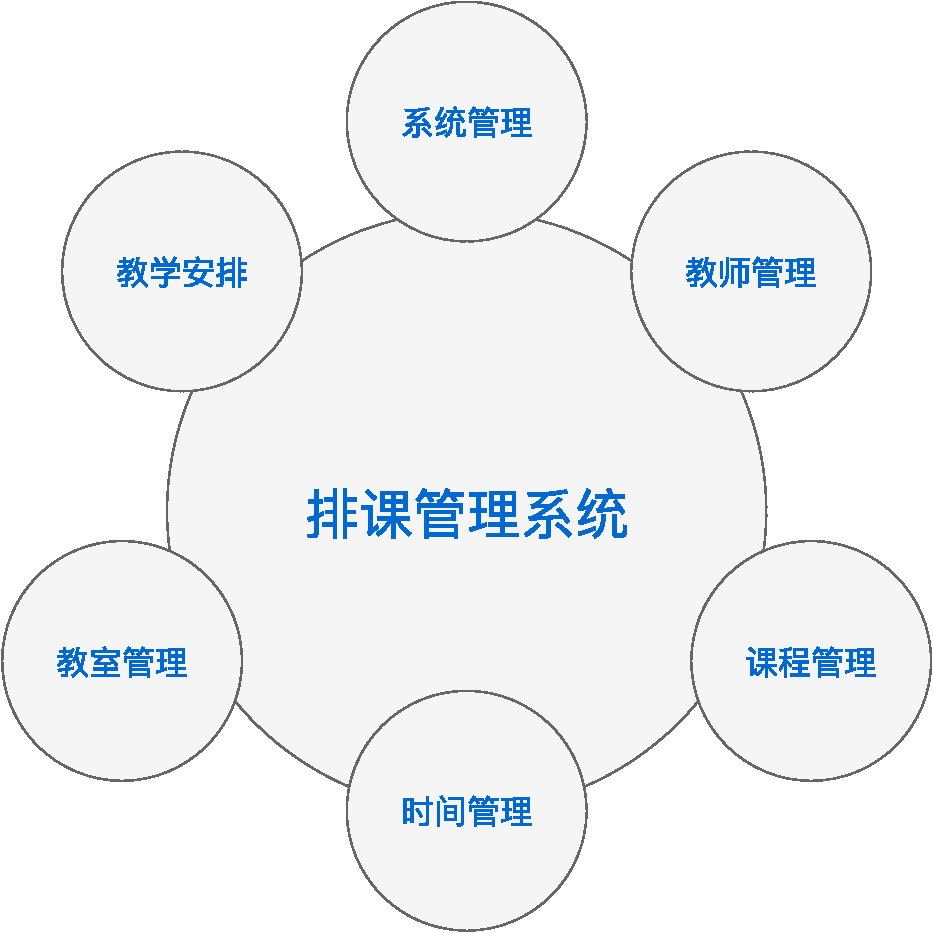
\includegraphics[width = 0.6\textwidth]{function}
      \caption{排课系统的管理功能}
      \label{fig:function}
    \end{figure}

  \subsection{业务流分析}
    \subsubsection{管理员业务}
      管理员业务如图\cref{fig:manager_function}
      \begin{figure}[H]
        \centering
        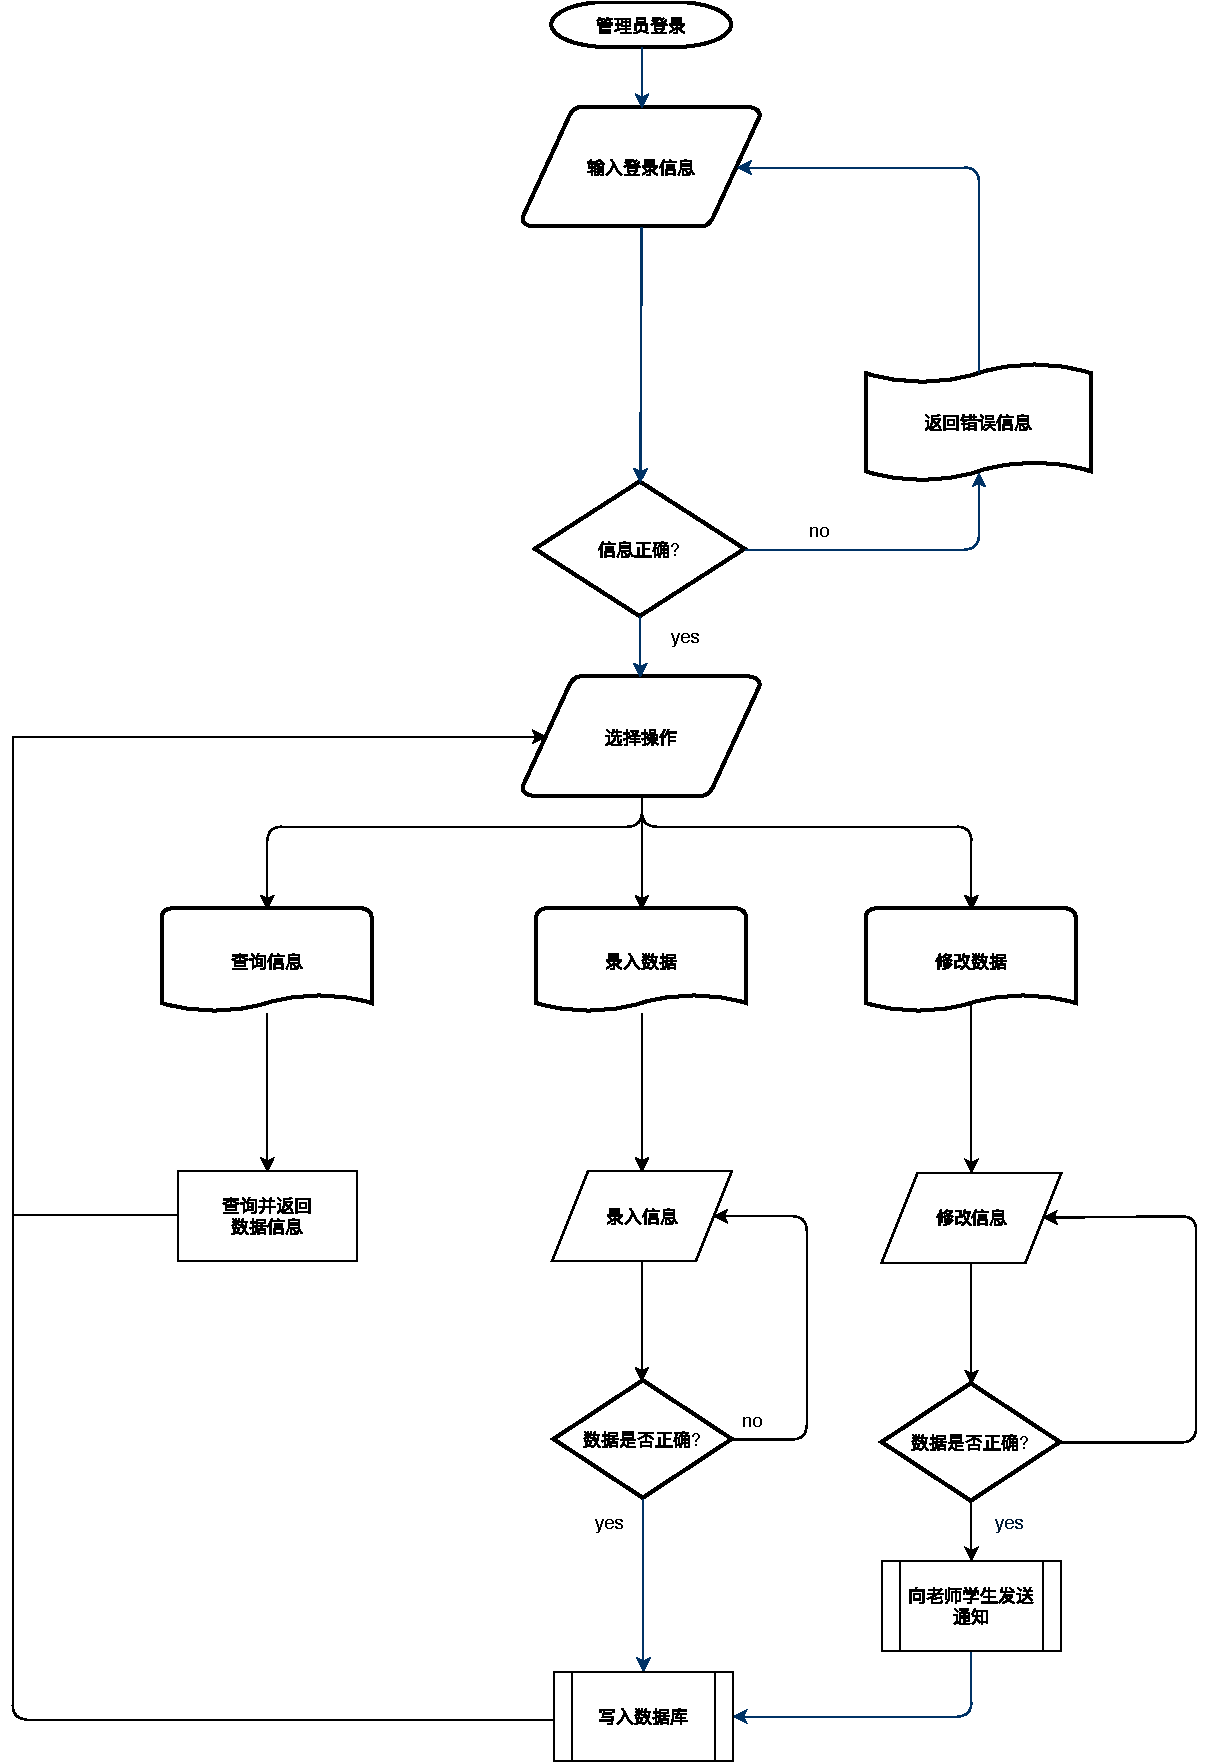
\includegraphics[width = 0.6\textwidth]{manager_function}
        \caption{管理员的业务流}
        \label{fig:manager_function}
      \end{figure}
    \subsubsection{教师查询}
      教师的业务如
      \cref{fig:teacher_function}
      \begin{figure}[H]
        \centering
        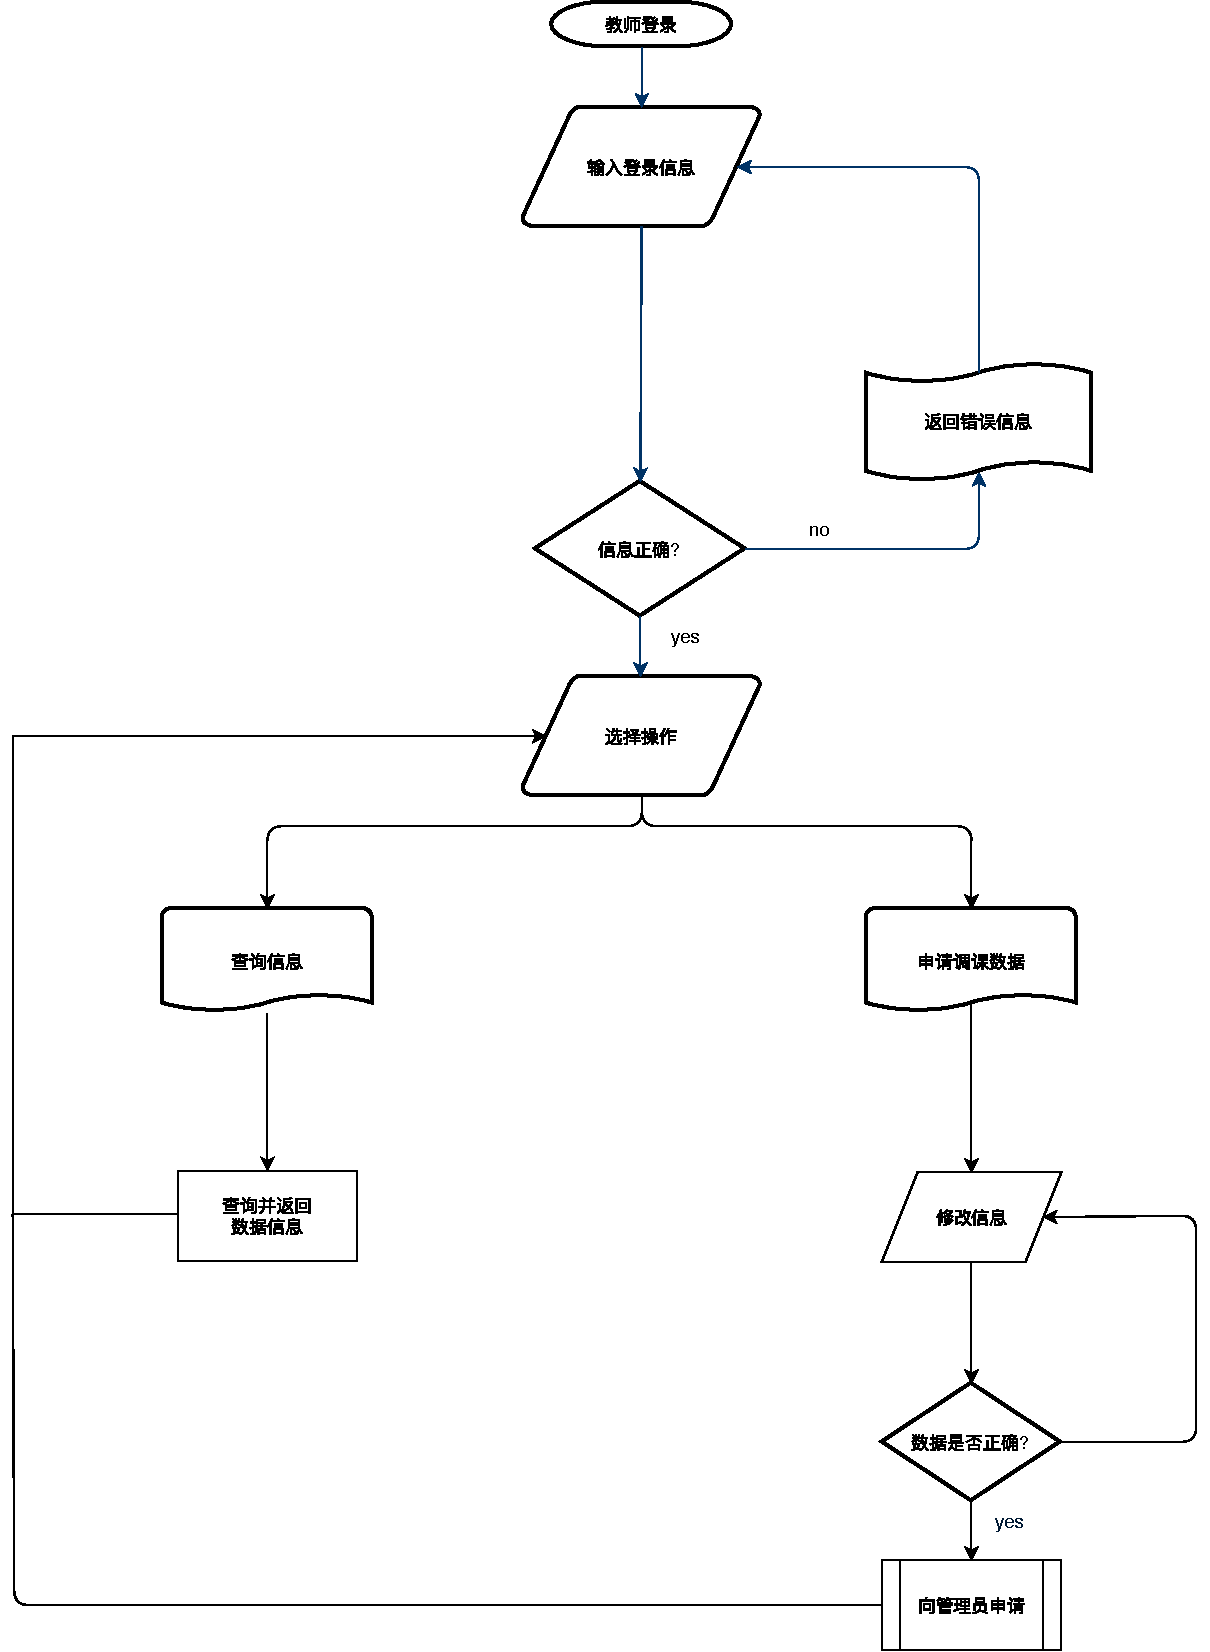
\includegraphics[width = 0.6\textwidth]{teacher_function}
        \caption{教师业务流程}
        \label{fig:teacher_function}
      \end{figure}

  \subsection{数据流分析}
    系统外部环境图如
    \cref{fig:outer}
    \begin{figure}[H]
      \centering
      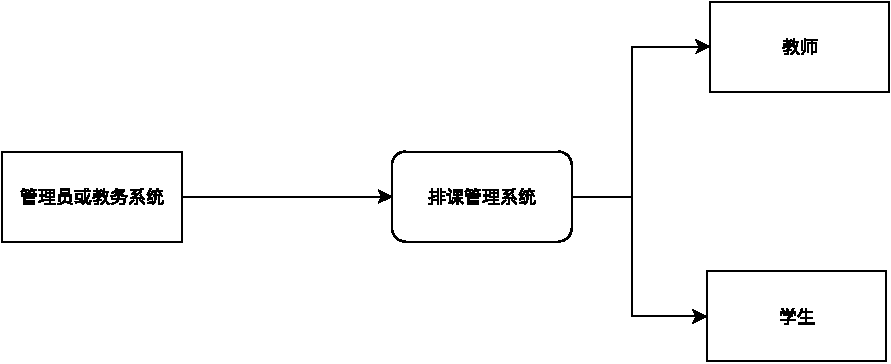
\includegraphics[width = 0.6\textwidth]{outer}
      \caption{系统外部环境图}
      \label{fig:outer}
    \end{figure}

    接下来将模型细化,
    \cref{fig:dataflow_1}
    描绘了系统的主要功能
    \begin{figure}[H]
      \centering
      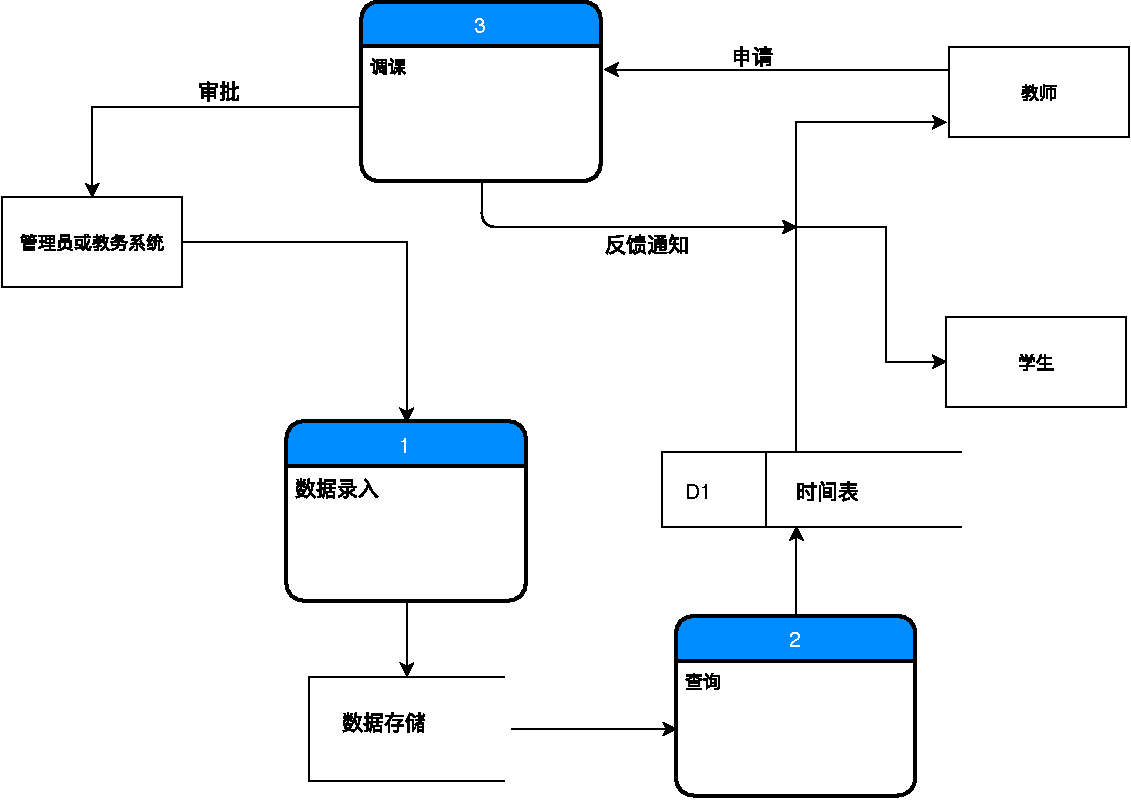
\includegraphics[width = 0.6\textwidth]{dataflow_1}
      \caption{排课系统功能的第一层数据流图}
      \label{fig:dataflow_1}
    \end{figure}

  \subsection{数据字典}
    \subsubsection{数据字典}

      根据数据流图中所涉及的信息,并对信息进行相应的分析,确定出所有数据项的描述内容,其主要分为数据项名称、类型、长度和取值范围,如\cref{t:data_dict}所示

      \begin{longtabu} to \textwidth {clcXXX}
        \caption{数据字典(具体的数据的大小参考\cite{tinyint})}
        \label{t:data_dict} \\
        \toprule[1.5pt]
          \makebox[0.1\textwidth]{名称}  &
          \makebox[0.2\textwidth]{含义} &
          \makebox[0.1\textwidth]{类型} &
          \makebox[0.1\textwidth]{大小} &
          \makebox[0.1\textwidth]{取值范围} &
          \makebox[0.2\textwidth]{备注} \\
        \midrule[1pt]
        \endhead

        \bottomrule[1.5pt]
        \endfoot


        % 表格正文
          楼号    & 教学楼的编号 & tinyint & \SI{1}{B} & 0-255 & \\
          楼名    & 教学楼的名称 & char(5) & \SI{15}{B} & 长度$\le 5$ & \\
          容量    & 教学楼的容量 & tinyint & \SI{1}{B} & 0-255 & \\
          院系编号 & 院系的编号 & tinyint & \SI{1}{B} & 0-255 & \\
          院系名   & 院系名 & char(8) & $\le\SI{24}{B}$ & 0-255 & \\
          课程号   & 课程编号 & char(20) & \SI{20}{B} & 20位 & \\
          课程名   & 课程名 & char(10) & $\le \SI{30}{B}$ & 10位 & \\
          类型名   & 课程的类型 & char(10) & $\le \SI{30}{B}$ & \\
          教师号   & 教师编号 & char(20) & \SI{20}{B} & 20位 & \\
          教师名   & 教师的姓名 & char(10) & $\le \SI{30}{B}$ & \\
          职称     & 教师的职称 & char(3) &\SI{9}{B}  & 助教, 讲师, 副教授, 教授 \\
          班号     & 班级编号 & char(20) & \SI{20}{B} & 20位 & \\
          班名     & 班级的全名 & char(10) & $\le \SI{30}{B}$ & \\
          人数     & 班级人数 & tinyint & \SI{1}{B} & 0-255 & \\
          时间号   & 上课时间的标识 & char(20) & \SI{20}{B} & 20位 & \\
          日       & 星期几 & tinyint & \SI{1}{B} & 0-255 & 星期用1-5代替\\
          开始时间 & 上课时间 & tinyint & \SI{1}{B} & 0-255 & 假设上课时间都是整点, 24小时制\\
          结束时间 & 下课时间 & tinyint & \SI{1}{B} & 0-255 & 假设下课时间都是整点, 24小时制\\
          开始周   & 第几周开始 & tinyint & \SI{1}{B} & 0-255 & \\
          结束周   & 第几周结束 & tinyint & \SI{1}{B} & 0-255 & \\
          is\_odd  & 单周上课 & bit & \SI{1}{B} & 0,1 & 默认为1 \\
          is\_even & 双周上课 & bit & \SI{1}{B} & 0,1 & 默认为1 \\
          节号      & 上课节的标识 & char(20) & \SI{20}{B} & 20位 & \\
          学期      & 在上学期或下学期 & bit & \SI{1}{B} & 0,1 & 每年第一学期为0,第二学期为1 \\
          年        & 年份 & smallint & \SI{2}{B} &$-32,768$- $32,767$ & \\

          % \specialrule{0em{8pt}{1pt}}
      \end{longtabu}
    \subsubsection{数据结构}

      根据数据流图中的信息的分析,在数据项描述的基础上确定所有数据结构的描述,
      主要有数据结构名称、含义和组成说明。
      本题数据结构如\cref{t:data_structure}.

      \begin{table}[H]
        \caption{数据结构说明}
        \label{t:data_structure}
        \centering
        \begin{tabularx}{\textwidth}{ccX}
        \toprule[1.5pt]
          \makebox[0.1\textwidth]{名称} &
          \makebox[0.4\textwidth]{含义} &
          \makebox[0.5\textwidth]{组成}  \\
          \midrule[1pt]
          $build$ & 教学楼信息 & 楼号, 楼名 \\
          $classroom$ & 教室信息 & 楼号, 教室号, 容量 \\
          $department$ & 院系 & 院系号, 院系名 \\
          $course$ & 课程信息 & 课程号, 课程名, 课程类型, 开课院系编号 \\
          $instructor$ & 老师信息 & 编号, 姓名, 职称, 院系编号, 研究方向 \\
          $class$ & 班级 & 班号, 班级名, 人数, 院系号 \\
          $time\_slot$ & 上课时间信息 & 时间标识符, 上课日, 上课时间, 下课时间, 开始周, 结束周, 单周上课, 双周上课 \\
          $section$ & 每节课的信息 & 课程编码,时间标识, 课程号, 学期, 开课年, 楼号, 教室号. \\



          % \specialrule{0em{8pt}{1pt}}
        \bottomrule[1.5pt]
        \end{tabularx}
      \end{table}

    \subsubsection{数据流描述}
      根据数据流图的数据流向的分析,确定所有数据流的描述,如
      \cref{t:dataflow}

      \begin{table}[H]
        \caption{数据流描述}
        \label{t:dataflow}
        \centering
        \begin{tabular}{cccc}
        \toprule[1.5pt]
          \makebox[0.2\textwidth]{数据流名} &
          \makebox[0.3\textwidth]{数据流来源} &
          \makebox[0.2\textwidth]{数据流去向} &
          \makebox[0.3\textwidth]{说明}
          \\
          \midrule[1pt]
          课程信息 & 管理员导入 & 学生,教师查询 & 记录每门课的信息 \\
          教师信息 & 管理员导入 & 学生,教师查询 & 记录教师的信息 \\
          教室信息 & 管理员导入 & 学生,教师查询 & 记录教室的信息 \\
          教学楼信息 & 管理员导入 & 学生,教师查询 & 记录教学楼的信息 \\
          调课申请 & 教师申请 & 管理员处理 & 调整上课信息 \\
          调课通知 & 管理员处理 & 学生,教师通知 & 调整上课信息 \\
          关注课程 & 学生,教师设置 & 用户自己查询 & 学生教师关注上课信息 \\
          个人课表 & 数据库 & 用户查询 & 可以设置显示关注课程 \\
          % \specialrule{0em{8pt}{1pt}}
        \bottomrule[1.5pt]
        \end{tabular}
      \end{table}

      \subsection{实体分析}

      \subsection{属性分析}

      \subsection{联系分析}

      \subsection{概念模型设计}
        % (.cdm图)

\section{数据库概念结构设计}
  \subsection{概念模型转化为逻辑模型}
    \subsubsection{一对一关系的转化}
      % (标注主、外键)

    \subsubsection{一对多关系的转化}

    \subsubsection{多对多关系的转化}

  \subsection{逻辑模型设计}
    % (.pdm图)



\section{数据库逻辑结构设计}
  \subsection{表设计}
    % (SQL server 中各表设计)

  \subsection{创建表和完整性约束代码设计}
    教学楼表定义:
    \begin{lstlisting}[language=sql]
      create table build(
        build_id tinyint,
        name char(5) not null,
        primary key (build_id),
      );
    \end{lstlisting}

    教室表定义:
    \begin{lstlisting}[language=sql]
      create table classroom(
        build_id tinyint,
        room_number smallint not null,
        capacity smallint,
        primary key (build_id, room_number),
        foreign key (build_id) references build,
      );
    \end{lstlisting}

  \subsection{创建视图、索引、存储过程和触发器}


\section{数据库的物理实现}

\section{数据库功能调试}
(包括视图、索引等内容的测试)

\section{应用程序设计}

\section{设计总结}





% 参考文献
\nocite{silberschatz1997database} % 数据库系统概论
\nocite{sqldbm} % 数据库画图软件
\nocite{pyqt5} % PyQt5 参考文档
\nocite{drawio}
\bibliography{reference} % 提示从reference数据库获取文献信息,来打印参考文献


\end{document}


% 命令用法
% % 插入代码
% \begin{lstlisting}[language=sql]
%   use university;
%   select * from university;
% \end{lstlisting}
